\chapter{陆地生态系统碳循环模型开放式对比框架}
\label{chap:arch}

陆地生态系统碳循环模型具有种类多样、参数复杂、难以应用的特点,模拟过程参与的要素众多(如GPP、NPP、NEP、Biomass、LAI等),模拟站点丰富,数据需求量大、难以搜集。这些因素都共同阻碍了碳循环模型的应用和发展,开展模型对比工作往往十分艰巨,像CMIP项目那样,各个模式开发组共同参与进来才能更顺利地完成。但是传统的对比框架也面临着一些问题,它将模型计算和对比过程都放在本地计算机运行,模型难以共享和重用,对比过程不够公开,换一套数据或研究区域就难以重现和重复,这些都是由于基于本地计算的对比框架所导致的。针对这一问题,本章旨在设计一个开放式的对比框架,支持将各种对比资源以微服务的形式开放地接入进来,实现可共享、可重用、公开化的陆地生态系统碳循环模型的对比。

本章首先分析了陆地生态系统碳循环模型的对比情景,并从中归纳总结出“对比话题——对比方案——对比任务”的三步流程;其次详细探讨了对比过程中的需要接入的地理资源组件库,包括有模型服务资源库、数据服务资源库、单位量纲资源库、数据处理服务资源库、对比服务资源库,并设计了对应接口来满足相应资源的接入,实现了对比资源的标准一致性和可扩展性;然后设计了分布式的网络系统架构,将整体复杂的系统功能分割为三部分,实现了功能的解耦和系统的稳定性;最后通过科学工作流引擎支持网络环境下对比流程地自动化执行。
本系统的整体架构如图\ref{fig:CMIP-architecture}所示。

\begin{figure}[!htbp]
    \centering
    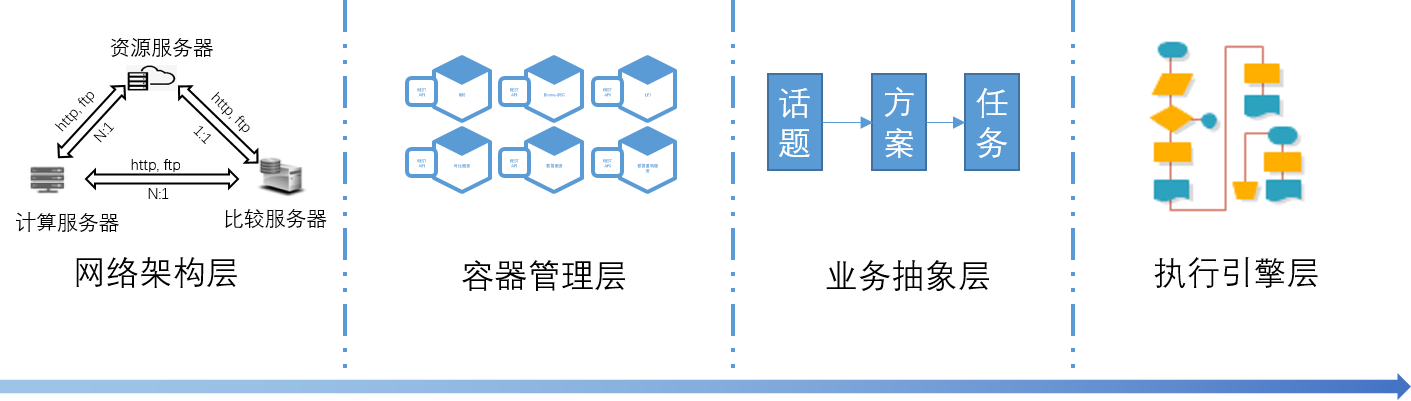
\includegraphics[width=1\textwidth]{CMIP-architecture}
    \caption{陆地生态系统碳循环模型开放式对比框架}
    \label{fig:CMIP-architecture}
\end{figure}

\section{陆地生态系统碳循环模型对比情景和业务分析归纳}
% 要不要放在第二章
\subsection{对比情景分析和总结}
\label{sec:scene}
% TODO 根据实验前提,详细介绍对比方案中的情景
陆地生态系统碳循环模型的应用广泛,未来的发展方向也主要停留在以下几个关键问题上:
\begin{enumerate}[(1)]
\item \textbf{陆地生态系统碳循环模型对历史植被生长的模拟}

在CMIP5和CMIP6的设计中,都设定了历史情景模拟,即根据历史时期的太阳常数、温室气体浓度、臭氧浓度、气溶胶浓度等观测资料来模拟气候因子,是气候系统模式参与CMIP项目的必要实验。而陆地生态系统碳循环模型作为气候系统模式机理中的一个子过程,也需要对历史时期进行模拟,来评估模型的模拟能力。历史情景分析是最常见的模拟情景,本文将在实验案例中详细介绍模拟结果。

\item \textbf{陆地生态系统碳循环模型的未来预测情景}
% 参考顾雪峰博士论文

在CMIP5和CMIP6中也设定了未来气候情景分析,即预测未来CO2浓度和气候因子(温度、降水)等指标的变化情况。在陆地生态系统碳循环模型对植被生产力的模拟方面,未来情景设定为百年后的气温、降水、CO2浓度的变化对植被生产力的影响,即研究陆地生态系统碳循环模型对气候变化(如温度、降水等)和CO2浓度的响应。CMIP5对未来100年全球气候变化的研究结果表明,全球平均气温从1990年到2100年上升$1.4\sim5.8^{\circ}C$~\cite{houghton2001climate}~\cite{王绍武1995未来}~\cite{秦大河2003气候变化的事实与影响及对策};全球平均降水将会增加,但是降水格局也发生了很大的变化,即有些地区降水增加,有些地区降水减少;未来大气CO2浓度最大升高到当前的2倍~\cite{griggs2002climate}。根据这些预测的未来气候情景,对温度、降水和CO2浓度的变化做出变量组合,表~\ref{tab:future-scene}可以表示一种参考的组合。

% \hspace*{2cm}
\begin{table}[!htbp]
    \centering
    \caption{陆地生态系统碳循环模型的未来预测情景参数设定}
    \label{tab:future-scene}
    \begin{threeparttable}
        \begin{tabular}{lll}
            \Xhline{2pt}
            {\textbf{因素}} & {\textbf{值}} & {\textbf{标记}} \\
            \Xhline{2pt}
            \multirow{4}{*}{\textbf{气温}} & 不变 & $Temp_{0}$ \\
            & +2$^{\circ}C$ & $Temp_{1}$ \\
            & +4$^{\circ}C$ & $Temp_{2}$ \\
            & +6$^{\circ}C$ & $Temp_{3}$ \\
            \hline
            \multirow{7}{*}{\textbf{降水}} & 不变 & $Prec_0$ \\
            & 全年+10\% & $Prec_{+10}$ \\
            & 全年-10\% & $Prec_{-10}$ \\
            & 全年+20\% & $Prec_{+20}$ \\
            & 全年-20\% & $Prec_{-20}$ \\
            & 全年+30\% & $Prec_{+30}$ \\
            & 全年-30\% & $Prec_{-30}$ \\
            \hline
            \multirow{2}{*}{\textbf{CO2浓度}} & 不变 & $CO2_0$ \\
            & 两倍 & $CO2_{*2}$ \\
            \hline
            \multirow{4}{*}{\textbf{多因素}} & 温度增加、降水增加 & $Temp_{3} + Prec_{+10}$ \\
            & 温度增加、降水减少 & $Temp_{3} + Prec_{-10}$ \\
            & 温度增加、降水增加、CO2浓度翻倍 & $Temp_{3} + Prec_{+10} + CO2_{*2}$ \\
            & 温度增加、降水减少、CO2浓度翻倍 & $Temp_{3} + Prec_{-10} + CO2_{*2}$\\
            \Xhline{2pt}
        \end{tabular}
    \end{threeparttable}
\end{table}

\item \textbf{陆地生态系统碳循环模型的敏感性分析情景}
% 和对温度、降水、CO2的响应比较像,这里针对的是模型参数

在模型评价中,不确定分析研究的是模型参数、驱动变量等不确定性因素发生变化时,所引起的模型模拟结果的变化和变化程度。敏感性分析是模型不确定分析的一种常用方法,它用来研究和预测不确定性因素发生变化时,对模型结果影响程度的分析方法,又称为灵敏度分析。敏感性分析通常用来评估模型参数的重要性,分为总体敏感性分析和局部敏感性分析。局部敏感性分析相对来说更加简单,他分析单个模型参数对模拟结果的影响,但是他忽略了模型之间多个参数的相互作用对模拟结果的影响;全局敏感性分析不仅分析单个参数对模拟结果的影响,还分析参数之间的相互作用对结果的总影响,但计算起来比较复杂,耗费时间。
在本文中,将敏感性分析也理解为一种对比情景,即在不同的模型参数下模拟结果的对比,可以与正常模拟与观测数据的对比采用相同的对比方法。敏感性分析的情景设定需要从每个模型中选出一系列关键参数,根据参数的取值设定具体的情景,由于本文的研究重点不在于此,不做详细设定。

\item \textbf{陆地生态系统碳循环模型的参数校准情景}

碳循环模型的模拟精确度很大成分上依赖于模型参数的设定,目前在参数校准方面有人工校准和自动校准两种。人工校准通常有三种方法:对比实验、实验观测和文献查找;自动校准通过神经网络等各种模型进行校准。模型参数的校准可以理解为在不同模型参数下模型模拟结果的对比,因此可以作为对比的一种情景。

\end{enumerate}

\subsection{对比业务抽象和归纳}
% 对比分析、名词解释
% topic solution task
% 案例
% 意义:可共享 可重用
% TODO 对比方案具体点:有观测数据、无观测数据

在进行对比业务抽象和归纳之前,先对本文中的一些名字做出解释:本文将GPP、NPP、NEP、Biomass、LAI等模拟指标称之为\textbf{对比要素};将模型对比过程中所需要的所有数据称之为\textbf{对比数据集},一套对比数据集包括有输入数据集、观测数据集。其中输入数据集由气象数据集、土壤数据集、植被功能类型数据集、DEM数据集等组成,每个具体的数据集可以选择可替换的模块,如气象数据集既可以采用MERRA 2再分析资料,又可以使用CRU再分析资料。在第\ref{sec:model-data}节中具体介绍的数据本文称之为标准对比数据集,作为系统分析的基础原始数据,而在其之上参照表~\ref{tab:future-scene}对数据进行的一系列修改,比如对温度$\pm2^{\circ}C$,对降水$\pm10\%$等,本文称之为衍生对比数据集。每一个模拟情景都有一套相对应的对比数据集。本文将参与对比的模型称之为\textbf{对比参与者}。

\begin{figure}[!htbp]
    \centering
    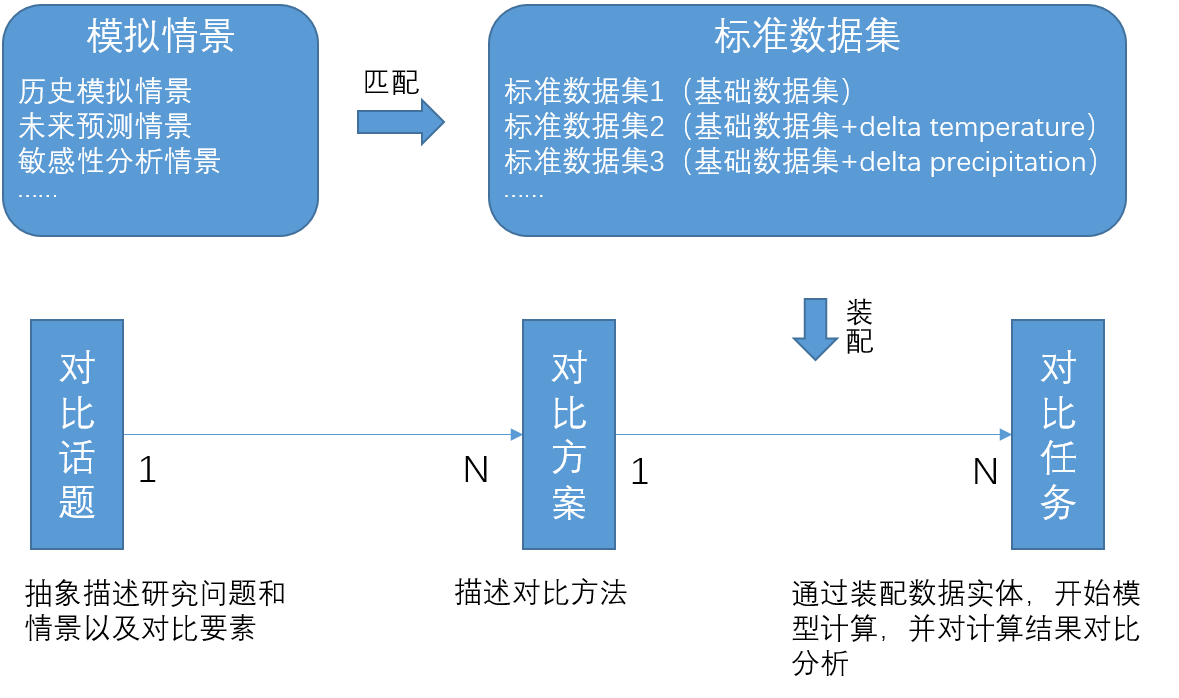
\includegraphics[width=1\textwidth]{cmip-business-abstraction}
    \caption{陆地生态系统碳循环模型对比业务抽象和归纳}
    \label{fig:cmip-business-abstraction}
\end{figure}

陆地生态系统碳循环模型在各种情景中可以归纳出三个主要关注点:研究问题、对比方法和模型运行数据的设定。这三点可以抽象为对比话题、对比方案和对比任务三个层次,如图~\ref{fig:cmip-business-abstraction}所示,对比业务的开展对应为对比话题、对比方案和对比任务创建和执行上。其中,\textbf{对比话题}中指明了研究问题、对比情景和对比要素;\textbf{对比方案}配置了对比参与者和对比方法,对比方案不包括具体的输入数据、观测数据和模拟结果,他表示的仅仅是对比的配置项,从而实现对比过程的可共享性、可重用性和可重现性;\textbf{对比任务}描述的是对比方案配置输入数据和观测数据实体的结果。模型在对比任务中开始具体的运算,并将运算结果与观测数据进行统计学对比和可视化对比。1个对比话题可以对应多个对比方案,一个对比方案通过配置不同的标准数据集可以对应多个对比任务。图~\ref{fig:ModelComparison!3-1-topic-solution-task_3}展示了对比话题、对比方案和对比任务的详细接口设计。

\begin{figure}[!htbp]
    \centering
    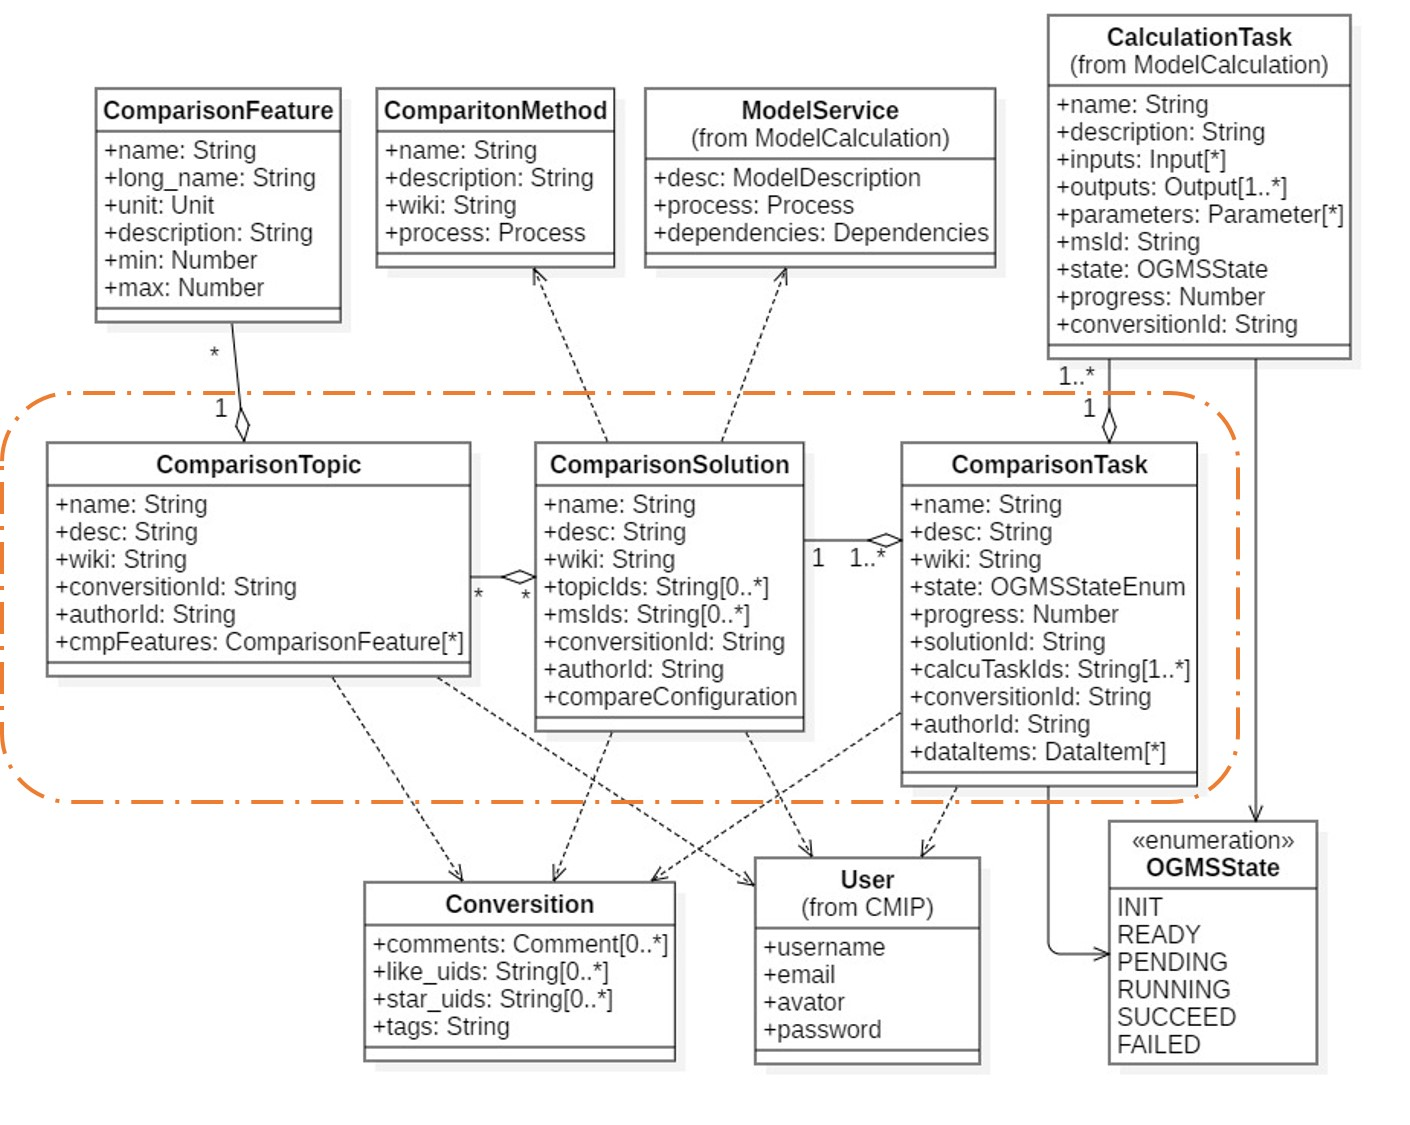
\includegraphics[width=1\textwidth]{jpg/ModelComparison!3-1-topic-solution-task_3}
    \caption{对比话题、对比方案和对比任务的接口设计UML图}
    \label{fig:ModelComparison!3-1-topic-solution-task_3}
\end{figure}

以植被生产力的对比为例,如表\ref{tab:topic-solution-task-example}所示,针对全球历史时期的植被生产力创建一个对比话题,对比要素包括有GPP、NPP、NEP等,这一个话题关联两个对比方案,其中对比参与者相同,都是IBIS、Biome-BGC和LPJ三个模型,第一个方案研究的是站点尺度,它使用的对比方法包括统计学和可视化两大类,通过配置不同的站点数据可以对应231个对比任务;第二个方案研究的是全球范围,它使用的对比方法只有可视化对比方法,只能创建一个相应的对比任务。这样的三层抽象使对比方案可共享与重用,简化了模型对比的难度,并将最后的对比结果公开发布为服务,使对比过程公开透明,更加具有可信度。

% TODO 从 pdf 导入吧
\begin{table}
    \centering
    \caption{针对全球植被生产力评估的对比话题、对比方案和对比任务}
    \label{tab:topic-solution-task-example}
    \begin{threeparttable}
        \begin{tabular}{l | l | l | l | l }
            \Xhline{1.5pt}
            \multicolumn{2}{c}{\makecell[b]{对比话题}} & \multicolumn{2}{|c|}{\makecell[b]{对比方案}} & \multicolumn{1}{l}{\makecell[b]{对比任务}} \\
            \hline
            模拟情景 & 对比要素 & \makecell{对比参与者} & \makecell{对比方法} & 数据区域 \\
            
            \Xhline{1.5pt}
            \multirow{3}{*}{历史情景} & \multirow{3}{2cm}{GPP \quad NPP \quad NEP\ } & \multirow{3}{*}{\makecell{IBIS\\Biome-BGC\\LPJ}} & \multirow{2}{*}{\makecell{统计学对比方法\\可视化对比方法}} & CN-Cha(长白山)站点 \\
            \cline{5-5}
            &  &  &  & 其他站点,共231个 \\
            \cline{4-5}
            &  &  & 可视化对比方法 & 全球 \\
            \Xhline{1.5pt}
        \end{tabular}
    \end{threeparttable}
\end{table}


\section{基于服务的地理资源组件库}
% 要不要和 微服务容器 放在一起
GIS的发展和信息技术的发展紧密关联,随着IT技术的不断推动,GIS经历了从集成式到组件式再到基于服务的Web GIS的发展历程,其中集成式GIS功能丰富全面但系统复杂、庞大、成本高昂,而且不能与其他系统集成;组件式GIS通过多元空间数据无缝集成技术(Seamless Integration of Multisource Spatial-data,SIMS)解决了多源异构数据的访问,并且具有可扩展、可共享和可重用能力,但是组件只能应用于本地计算机;基于Web Service的Web GIS则通过定义空间数据和模型的标准描述协议,实现了数据、模型及计算资源的共享,具备可扩展性、跨平台性,使GIS真正实现大众化。

Web Service是一种服务导向架构的技术,通过Web协议提供服务,可以保证不同平台的应用程序之间可以互操作。Web Service的实现方式一般有简单对象访问协议(Simple Object Access Protocol,SOAP)和表述性状态转移(Representational State Transfer,REST)两种。REST服务在服务注册量、普及程度、响应时间、吞吐量和数据传输方面的性能都要优于SOAP服务~\cite{2015互联网上基于},因此本文选择REST服务作为技术支撑。REST服务基于HTTP协议之上,通过定义一种软件架构风格,以HTTP请求的POST、DELETE、GET和PUT方法对应对资源的增删查改操作~\cite{fielding2000architectural}。REST服务的特点是客户端——服务器端(Client-Server)架构、无状态、接口统一、系统分层等。
使用REST服务接入地理资源组件,实现了各种组件的可扩展性。

\subsection{模型服务资源库}
由于模型资源在编程语言(如C++、C\#、JAVA等)、存在形式(如源代码、可执行程序、DLL等)、运行交互方式(如控制台应用程序、GUI、网络服务等)、运行平台(如Windows、Linux、Unix等)等方面存在着很强的异构性,模型本身很难作为组件接入到框架下,对模型进行封装可以屏蔽这些异构性,形成标准化的模型服务。模型服务资源库由这些标准化的服务组成,它的应用模式如图~\ref{fig:model-operation}所示,其中每一步都通过HTTP协议传输,其详细接口设计如表~\ref{tab:model-service-API}所示。

其中模型调用接口“/model-service/:msId/invoke”是最重要的,其请求参数如表~\ref{tab:model-invoke-API}所示,输入项、参数项、输出项的id从“/model-service/:msId”接口返回的描述文档中可以获取,输入项的“value”是上传到服务器返回的数据id,参数项的“value”是Number或String类型的值,输出项的“value”不用填写。发送请求后,如果调用成功,则返回运行记录的id,凭此id可以通过“/model-service/record/:recordId”接口请求模型的运行记录,并从中获取运算的结果。

模型服务资源库屏蔽了模型的异构性,简化了模型的使用难度,不同的模型资源具有相同的地位和角色,都看作为对比参与者,在对比框架下,能够可扩展地加入到对比方案中。

\begin{figure}[!htbp]
    \centering
    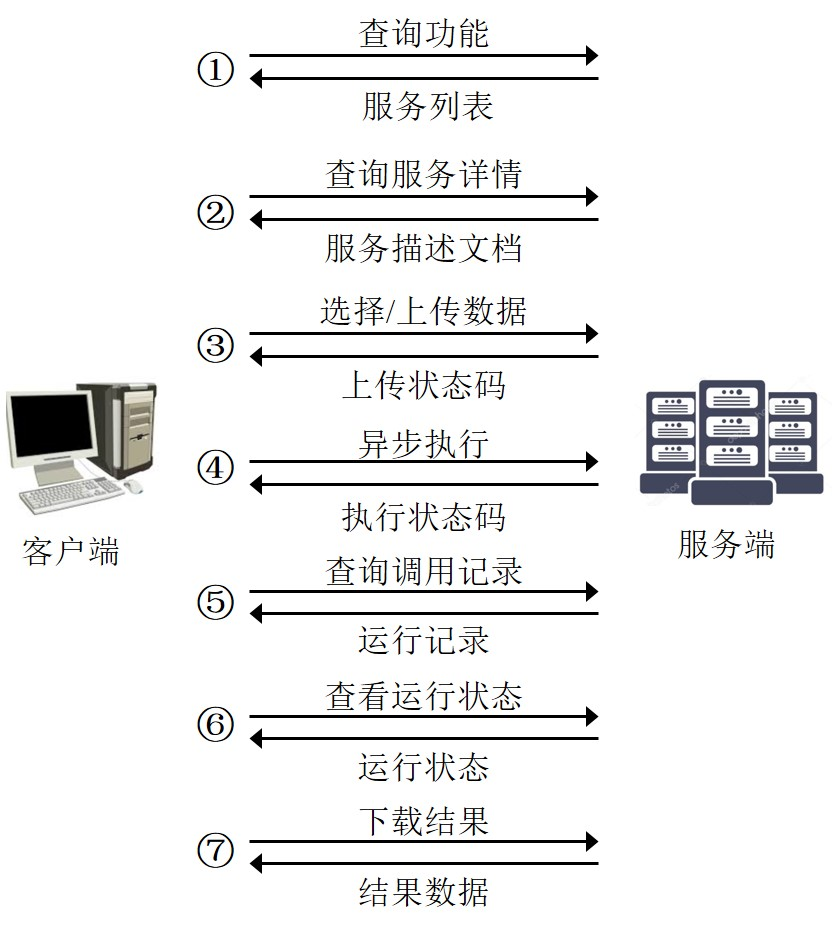
\includegraphics[width=.8\textwidth]{model-operation}
    \caption{模型服务交互模型}
    \label{fig:model-operation}
\end{figure}

\begin{table}[!htbp]
    \centering
    \caption{模型服务API}
    \label{tab:model-service-API}
    \begin{tabular}{llll}
        \Xhline{1.5pt}
        名称 & 请求方式 & 返回 & 说明 \\
        \Xhline{1.5pt}
        /model-service & GET & 模型服务列表 & 查询模型服务 \\
        /model-service/:msId & GET & 模型描述文档 & 查询模型详情 \\
        /model-service/:msId/invoke & POST & 状态码 & 运行模型 \\ 
        /model-service/record & GET & 运行记录列表 & 查询模型运行记录 \\
        /model-service/record/:recordId & GET & 运行记录 & 查询运行记录 \\
        \Xhline{1.5pt}
    \end{tabular}
\end{table}

\begin{table}[!htbp]
    \centering
    \caption{模型调用接口请求参数}
    \label{tab:model-invoke-API}
    \begin{tabular}{lll}
        \Xhline{1.5pt}
        参数 & 结构 & 描述 \\
        \Xhline{1.5pt}
        inputs 
        & 
        % \begin{minted}[tabsize=4]{js}
        $\{ "id": "data\_flag", "value": "data\_id\_you\_had\_uploaded" \}[]$
        % \end{minted}
        & 输入数据列表 \\
        parameters 
        &
        % \begin{minted}[tabsize=4]{js}
        $\{ "id": "data\_flag", "value": "parameter\_value" \}[]$
        % \end{minted}
        & 参数列表 \\
        outputs 
        &
        % \begin{minted}[tabsize=4]{js}
        $\{ "id": "data\_flag", "value": null \}[]$
        % \end{minted}
        & 输出数据列表 \\
        \Xhline{1.5pt}
    \end{tabular}
\end{table}

\subsection{数据服务资源库}
数据服务资源库由数据下载服务、数据重构服务和OGC WMS、WFS、WCS三类组成。其中数据下载服务将数据按照多种分类体系发布出去,并提供数据的相关元数据描述文档。数据在模型运行和对比时,往往并不能直接驱动程序的运行,数据重构服务对数据做出转换,它的调用交互模式和模型服务的调用类似,表~\ref{tab:data-service-API}列出了数据服务的详细接口,OGC WMS、WFS、WCS服务的接口和发布在后文第~\ref{subsubsec:OGC}节详细介绍。

\begin{table}[!htbp]
    \centering
    \caption{数据服务API}
    \label{tab:data-service-API}
    \begin{tabular}{llll}
        \Xhline{1.5pt}
        名称 & 请求方式 & 返回 & 说明 \\
        \Xhline{1.5pt}
        /data & POST & 状态码和数据id & 上传数据 \\
        /data & GET & 数据列表 & 获取数据列表 \\
        /data/:dataId & GET & 数据文件 & 下载数据 \\
        /data/:dataId/metadata & GET & 元数据文档 & 获取元数据 \\
        /data-refactor & GET & 数据重构服务列表 & 查询数据重构服务 \\
        /data-refactor/:id & GET & 重构服务描述 & 查询重构服务详情 \\
        /data-refactor/:id/invoke & POST & 状态码 & 运行重构服务 \\
        /data-refactor/record & GET & 运行记录列表 & \multicolumn{1}{m{0.3\columnwidth}}{查询重构服务运行记录} \\
        /data-refactor/record/:recordId & GET & 运行记录 & 查询运行记录 \\
        \Xhline{1.5pt}
    \end{tabular}
\end{table}

\subsection{单位量纲资源库}
单位量纲资源库由模型运算过程中涉及到的单位和量纲组成,如图~\ref{fig:ModelComparison!3-2-unit-dimension_5}所示,量纲类Dimension由7个基本物理量组成,他们分别是长度($L$)、质量($M$)、时间($T$)、电流($I$)、温度($\Theta$)、物质的量($N$)、发光强度($J$)。而单位类Unit则由这7个基本物理量组合表示(对于无量纲的单位为空),它也可以是自定义的单位。在对比要素类ComparisonFeature中用单位来表达它的具体物理意义,对于不同的单位表示法,可以通过量纲分析进行换算。单位量纲只有一个接口,以GET方式请求“/metrics”可以获取单位量纲列表。表~\ref{tab:std-metrics}列出了本文涉及到的对比要素及其所使用的单位。

模型在对比时模拟数据和观测数据的单位量纲一般不完全相同,以GPP为例,IBIS的输出单位是$gC m^{-2} d^{-1}$,Biome-BGC的输出单位是$kgC m^2 d^{-1}$,观测数据的单位是$gC m^{-2} d^{-1}$,在对比时,需要将单位一致化,单位量纲资源库为单位转换提供参考。

\begin{figure}[!htbp]
    \centering
    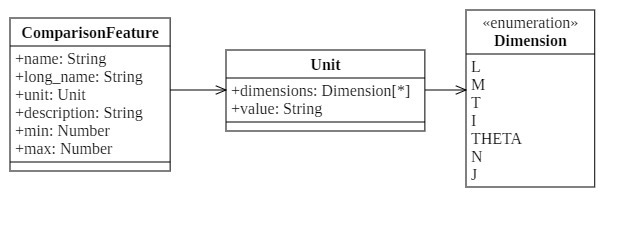
\includegraphics[width=.9\textwidth]{jpg/ModelComparison!3-2-unit-dimension_5}
    \caption{单位量纲UML图}
    \label{fig:ModelComparison!3-2-unit-dimension_5}
\end{figure}

% TODO min and max
\begin{table}[!htbp]
    \caption{对比要素及其单位量纲}
    \label{tab:std-metrics}
    \begin{subtable}[t]{.6\linewidth}
        \centering
        \caption{陆地生态系统碳水循环要素表}
        \label{tab:c-w-feature}
        \begin{tabular}{llrrr}
            \Xhline{1.5pt}
            \textbf{名称} & \textbf{单位} & \textbf{最小值} & \textbf{最大值}  \\
            \Xhline{1.5pt}
            $GPP$ & $gC m^{-2} d^{-1}$ & 0 & 100 \\
            $NPP$ & $gC m^{-2} d^{-1}$ & 0 & 100 \\
            $NEP$ & $gC m^{-2} d^{-1}$ & -100 & 100 \\
            $NEE$ & $gC m^{-2} d^{-1}$ & -100 & 100 \\
            $Biomass$ & $gC m^{-2} d^{-1}$ & 0 & - \\
            $R_A$ & $gC m^{-2} d^{-1}$ & 0 & 100 \\
            $R_H$ & $gC m^{-2} d^{-1}$ & 0 & 100 \\
            $ET$ & $mm d^{-1}$ & 0 & 100\\
            $Runoff$ & $mm d^{-1}$ & - & - \\
            $LAI$ & $m^2/m^2$ & 0 & 1 \\
            \Xhline{1.5pt}
        \end{tabular}
    \end{subtable}%
    \begin{subtable}[t]{.3\linewidth}
        \centering
        \caption{单位量纲表}
        \label{tab:unit-dimension}
        \begin{tabular}{ll}
            \Xhline{1.5pt}
            \textbf{单位} & \textbf{量纲}  \\
            \Xhline{1.5pt}
            \multirow{3}{*}{$gC m^{-2} d^{-1}$} & 质量($M$) \\
            & 长度($L$) \\
            & 时间($T$) \\
            \hline
            \multirow{3}{*}{$kgC m^{-2} y^{-1}$} & 质量($M$) \\
            & 长度($L$) \\
            & 时间($T$) \\
            \hline
            \multirow{2}{*}{$mm d^{-1}$} & 长度($L$) \\
            & 时间($T$) \\
            \Xhline{1.5pt}
        \end{tabular}
    \end{subtable}
\end{table}

\subsection{对比服务资源库}
对比服务资源库分为两类:统计学对比方法和可视化对比方法。他们都接受一条或多条数据为输入,统计学对比方法返回的是统计指标,可视化对比方法返回的是图片结果。表~\ref{tab:cmp-service-API}列出了去详细接口。

\begin{table}[!htbp]
    \centering
    \caption{对比服务API}
    \label{tab:cmp-service-API}
    \begin{tabular}{llll}
        \Xhline{1.5pt}
        名称 & 请求方式 & 返回 & 说明 \\
        \Xhline{1.5pt}
        /cmp & GET & 对比服务列表 & 查询对比服务 \\
        /cmp/:cmpId & GET & 对比服务描述文档 & 查询对比服务详情 \\
        /cmp/:cmpId/invoke & POST & 状态码 & 运行对比服务 \\ 
        /cmp/record & GET & 对比记录列表 & 查询对比服务运行记录 \\
        /cmp/record/:recordId & GET & 对比结果 & 查询对比结果 \\
        \Xhline{1.5pt}
    \end{tabular}
\end{table}

\section{基于微服务的分布式网络架构设计}
% 开放性应体现在:可共享和重用(业务流程归纳)、计算和对比过程公开化(服务化)、模型和数据资源可扩展(微服务注册和发现)、大规模计算场景下体系稳定可用(微服务LB)、自动化易用(科学工作流)
\subsection{微服务简介与应用}
% 使用原因-引入微服务
% 简介、特点、优点
% 本文应用详细介绍
分布式系统是由一组通过网络进行通信、为了完成共同的任务而协调工作的计算机节点组成的系统。分布式将不同物理区域的计算资源组织整合起来,与传统的集中式相对比,分布式能够有效利用多个分布式节点上的计算能力和数据共享能力,从而提高服务端的性能。
微服务是一种分布式的系统架构风格,由Martin Fowler提出~\cite{fowler2014microservices},微服务是颗粒比较小的服务,服务之间相互独立,具有其独自的数据管理,可以被独立部署,一个大型的复杂软件可以由多个微服务组成。微服务采用UNIX的设计哲学,每种服务只做一件事,是一种松耦合的能够被独立开发和部署的无状态化服务。微服务通过服务来实现应用的组件化,微服务中将组件定义为可被独立替换和升级的软件单元,在应用架构设计中通过将整体应用切分成可独立部署的多个微服务方式进行组件化设计。

\begin{figure}[!htbp]
    \centering
    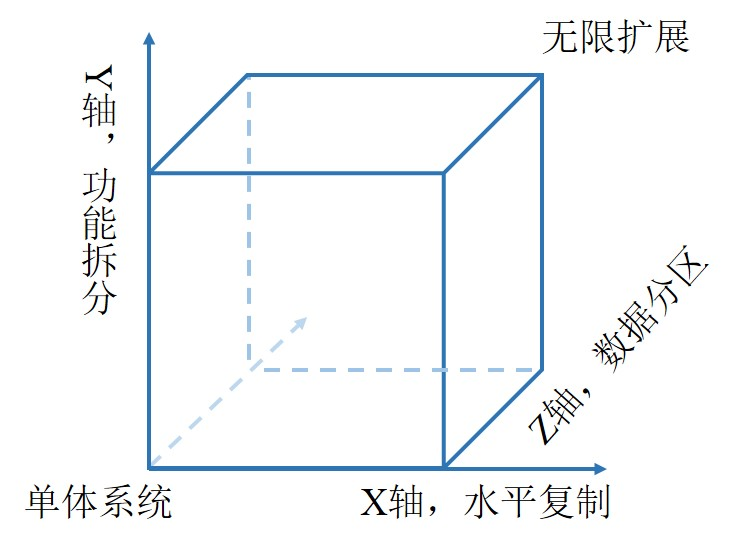
\includegraphics[width=.35\textwidth]{AKF-cube}
    \caption{AKF扩展立方体模型}
    \label{fig:AKF-cube}
\end{figure}

\begin{figure}[!htbp]
    \centering

    \subcaptionbox{微服务应用架构\label{micro-arch}}{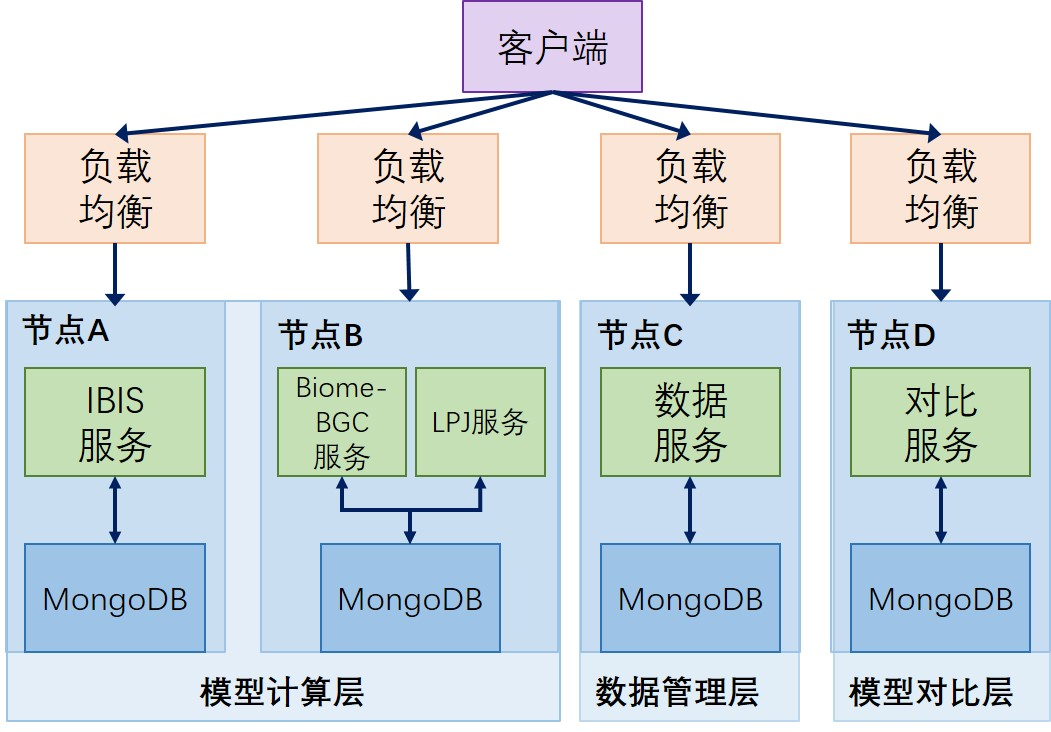
\includegraphics[width=0.6\textwidth]{multi-arch}}
    \hfill
    \subcaptionbox{单体服务应用架构\label{single-arch}}{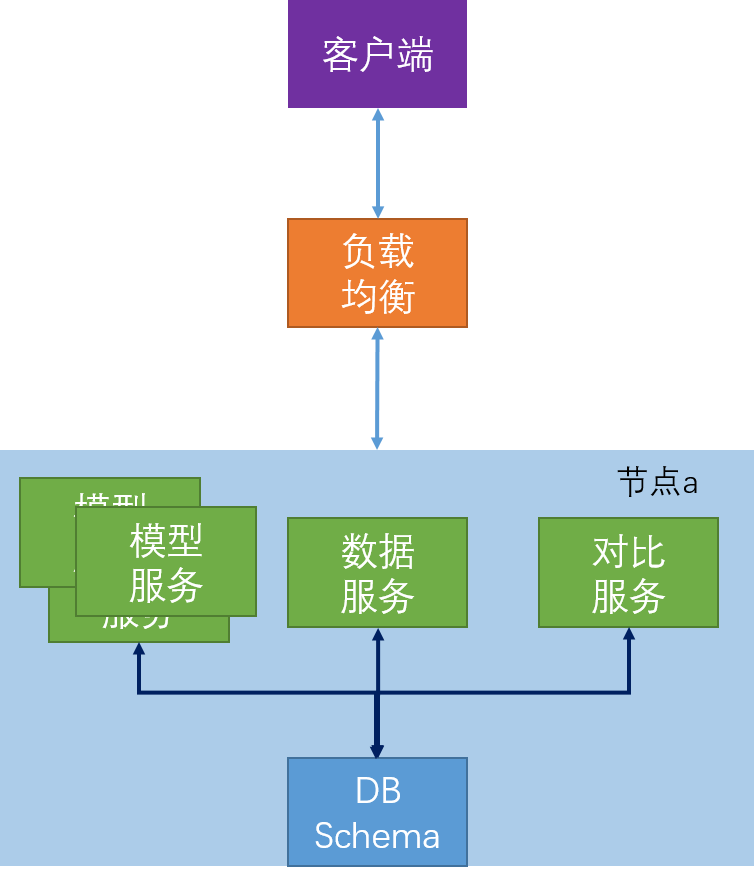
\includegraphics[width=0.35\textwidth]{single-arch}}

    \caption{微服务架构与单体服务架构的对比}
    \label{fig:ms-server-microservice}
\end{figure}

如图~\ref{fig:AKF-cube}所示,微服务的特点可以用AKF立方体~\cite{abbott2009art}表示,应用程序的开发可以抽象为三个维度:

\begin{enumerate}[(1)]
    \item \textbf{X轴:}水平复制。将单体系统运行多个实例,并在其间做负载均衡;
    \item \textbf{Y轴:}功能拆分。基于不同的业务将功能划分为不同的微服务;
    \item \textbf{Z轴:}数据分区。对应用程序的数据库进行拆分,避免遇到数据库瓶颈。
\end{enumerate}

理论上按照这三个维度的扩展模式,可以将单体系统进行无限扩展。

如图~\ref{micro-arch}所示,本文将整个对比工作分为模型计算、数据存储和模型对比三大部分,每一部分划分为微服务实现,其中模型微服务根据模型的软硬件需求,可以将多个模型部署在同一台计算机上,也可以单独部署,由于IBIS模型计算较慢,对软硬件需求较高,本文把他独立部署在一台节点上,而Biome-BGC和LPJ相对来说计算很快,将他们部署在一起。
图~\ref{single-arch}展示了传统的单体服务架构,它将所有功能需求都放在同一台服务器上实现,使得系统庞大臃肿,任意模块一旦崩溃都会引起整个系统的崩溃,而与之相比微服务效率高、灵活性强、可用性高、可扩展性强。
% \begin{figure}[!htbp]
%     \centering
%     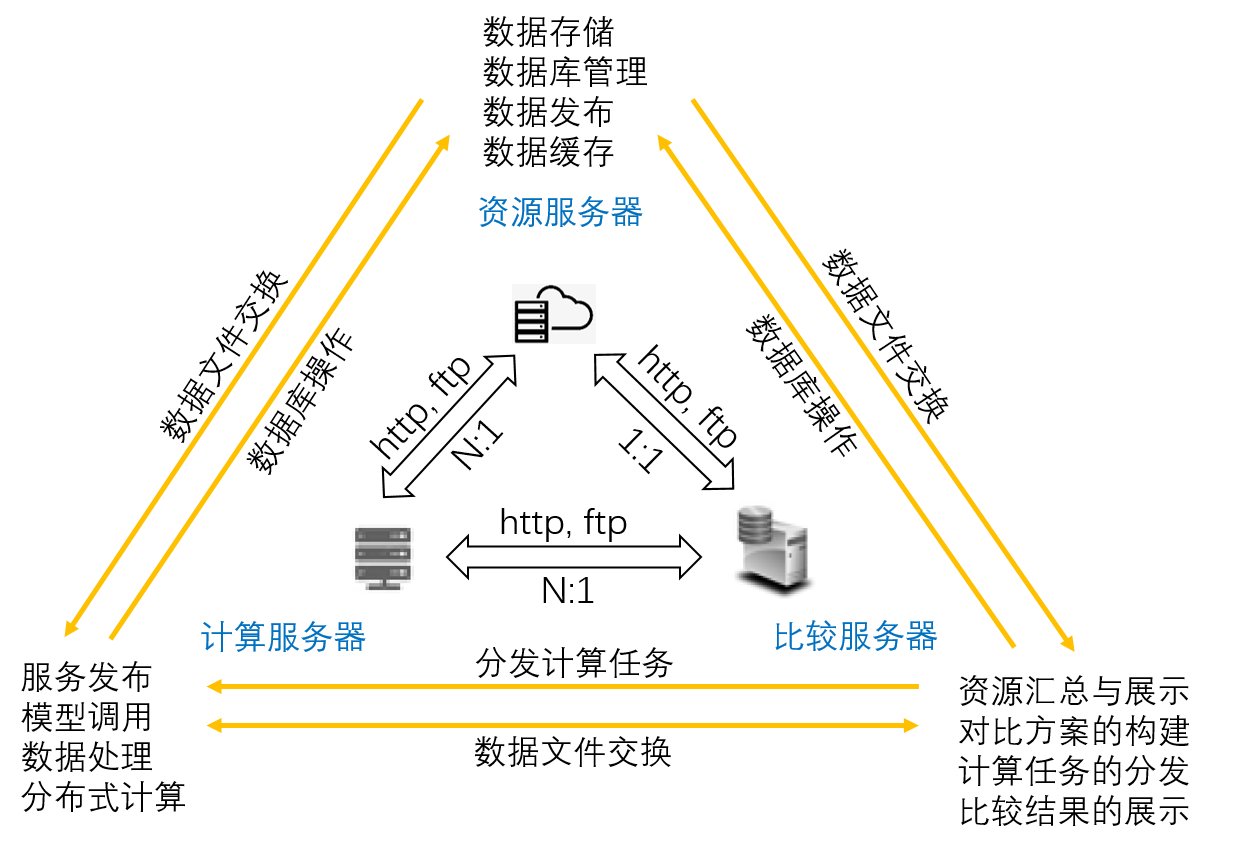
\includegraphics[width=1\textwidth]{network-archecture}
%     \caption{分布式网络架构}
%     \label{fig:network-archecture}
% \end{figure}

\subsection{服务治理}
% 微服务带来的一系列问题,如何解决
微服务通过功能分解为系统带来无限扩展的可能,通过功能分解带来优点的同时在集成时也面临着一系列的问题,比如如何发现服务?如何统一对服务进行认证管理?如何针对对比需求进行服务集成?这些都是需要解决的问题。
\subsubsection{动态服务注册与发现}
传统的单体应用之间耦合关系较少,通过手动配置IP地址和端口就能满足需求,但是在微服务架构下,服务提供者会不断扩展而变得越来越多,手动配置的方式并不适用于此,而是通过服务注册来解决。本文设计的注册分两个层级,如图~\ref{fig:service-registe-discover}所示,第一级是在计算节点内部的注册,由计算节点自己独立管理,比如模型计算节点可以发布一个或多个模型服务,也可以注销某些模型服务;第二级是将计算节点注册到中心服务器的数据库中,在计算节点启动时,自动向中心服务节点发送注册请求,并持续发送心跳,当计算节点宕机或手动注销时,心跳停止,中心服务器能够实时更新出注册的节点列表。

\begin{figure}[!htbp]
    \centering
    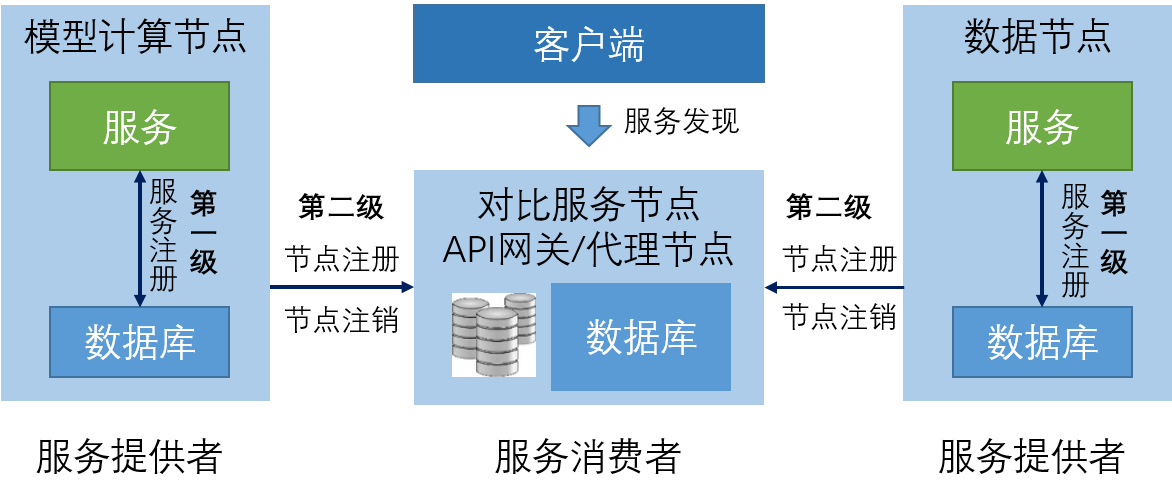
\includegraphics[width=.9\textwidth]{service-registe-discover}
    \caption{动态服务注册与发现}
    \label{fig:service-registe-discover}
\end{figure}

\subsubsection{API网关}
API网关也是针对微服务而出现的技术手段,在单体应用中,客户端需要请求的后台服务器只有一台,而微服务架构下,需要连接的后台节点就多种多样了,他们往往具有异构的接口、协议,以及许多重复化的功能单元(如认证),这大大增加了客户端逻辑的复杂度。如图~\ref{fig:API-gateway},API网关的设计则是在这些服务节点之上做出一次代理或简单处理,从而屏蔽微服务之间的异构性,使客户端感觉不到微服务的存在。此外,不同的微服务可以通过API网关共同管理其会话状态,从而达到状态共享的目的。在本系统中,API网关和模型对比服务器是同一个实体,在模型对比服务器上,对模型计算服务、数据服务进行服务集成,并做出负载均衡优化。

\begin{figure}[!htbp]
    \centering
    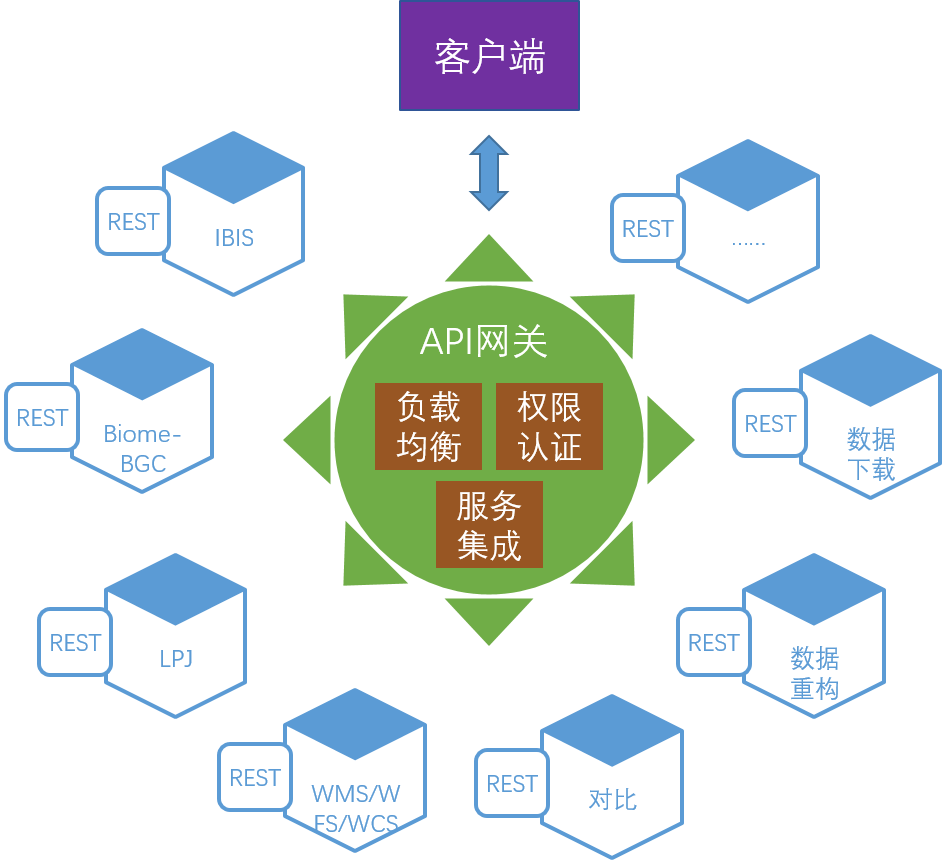
\includegraphics[width=.65\textwidth]{API-gateway}
    \caption{API网关}
    \label{fig:API-gateway}
\end{figure}

\subsection{微服务容器设计}
% 通用微服务容器
% 各个具体的容器的特点
本文将微服务容器定义为微服务的承载工具,具体体现是对应的后台服务器提供商。根据微服务的划分,将微服务容器划分为三类:数据管理容器、模型计算容器和模型对比容器。这三者有通用的功能:都对自己所承载的微服务进行管理,具体包括服务发布、服务注销、服务实例管理、性能监控等。此外,数据管理容器负责数据相关操作,包括数据存储、数据服务的发布和结果数据的缓存;模型计算容器负责模型服务的发布、注册、管理和调用;模型对比容器作为门户网站的后台服务器,负责资源的汇总与展示、对比话题和方案的创建、计算任务的分发和对比结果的展示。其中模型计算容器对外提供模型微服务,数据管理容器对外提供数据微服务,模型对比容器对外提供模型对比微服务,三者通过资源交换和消息通信完成协同完成对比任务。
\subsubsection{数据管理容器}
% 功能、特点、服务
数据服务容器主要有以下两点功能:
\begin{enumerate}[(1)]
\item \textbf{数据文件存储和缓存:}数据文件包括各种输入数据、对比参照数据和输出数据。模型在运行时从数据管理容器请求输入数据,运行结束后将输出数据存储到数据管理容器。对比任务执行时从数据管理容器请求模型输出数据和对比参考数据,并将对比结果的图表存储到数据服务容器;
\item \textbf{数据服务的发布:}包括WMS、WFS、WCS、下载服务、上传服务、数据重构服务具体参考第~\ref{sec:data-service}节。
\end{enumerate}

数据管理容器的硬件配置要求是硬盘大,网络带宽高,以方便数据存储和交换。

% \begin{figure}[!htbp]
%     \centering
%     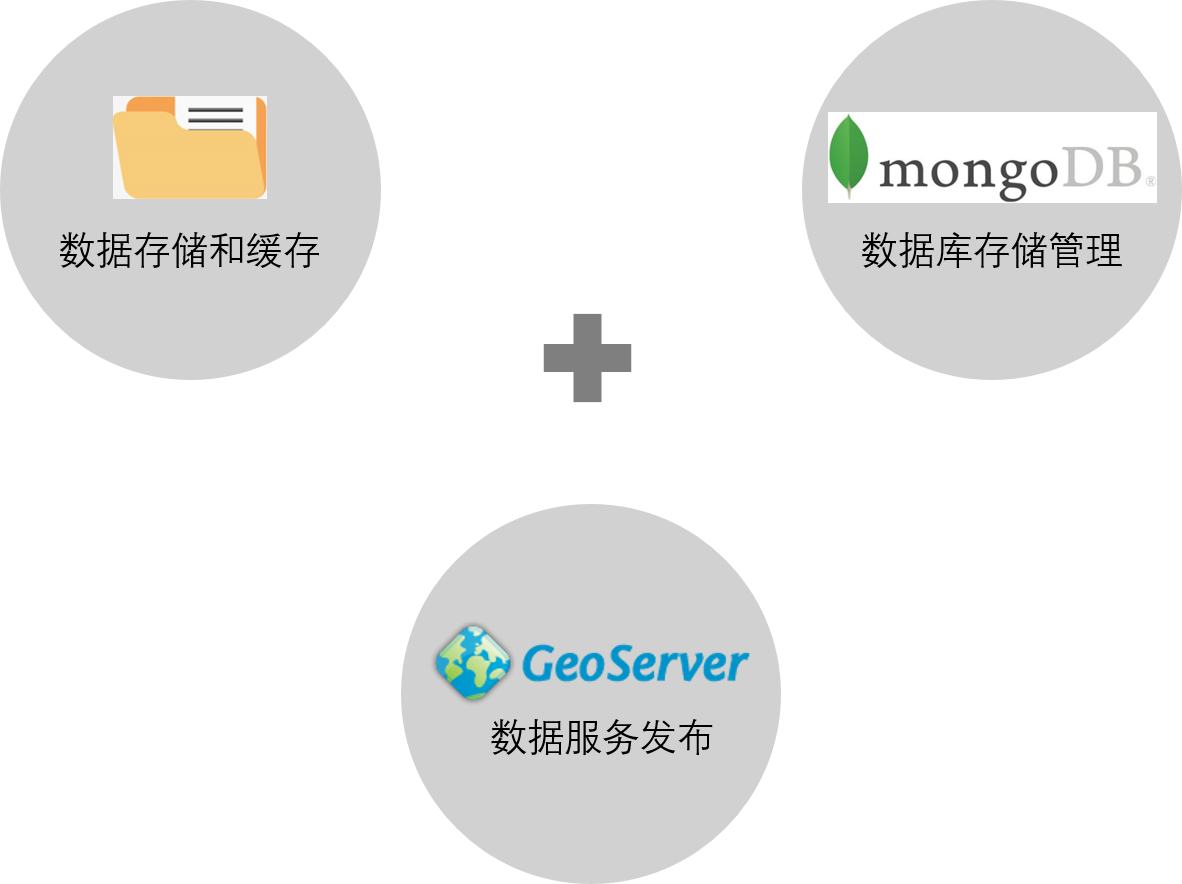
\includegraphics[width=1\textwidth]{resource-server}
%     \caption{数据管理容器功能}
%     \label{fig:resource-server}
% \end{figure}

% \begin{figure}[!htbp]
%     \centering
%     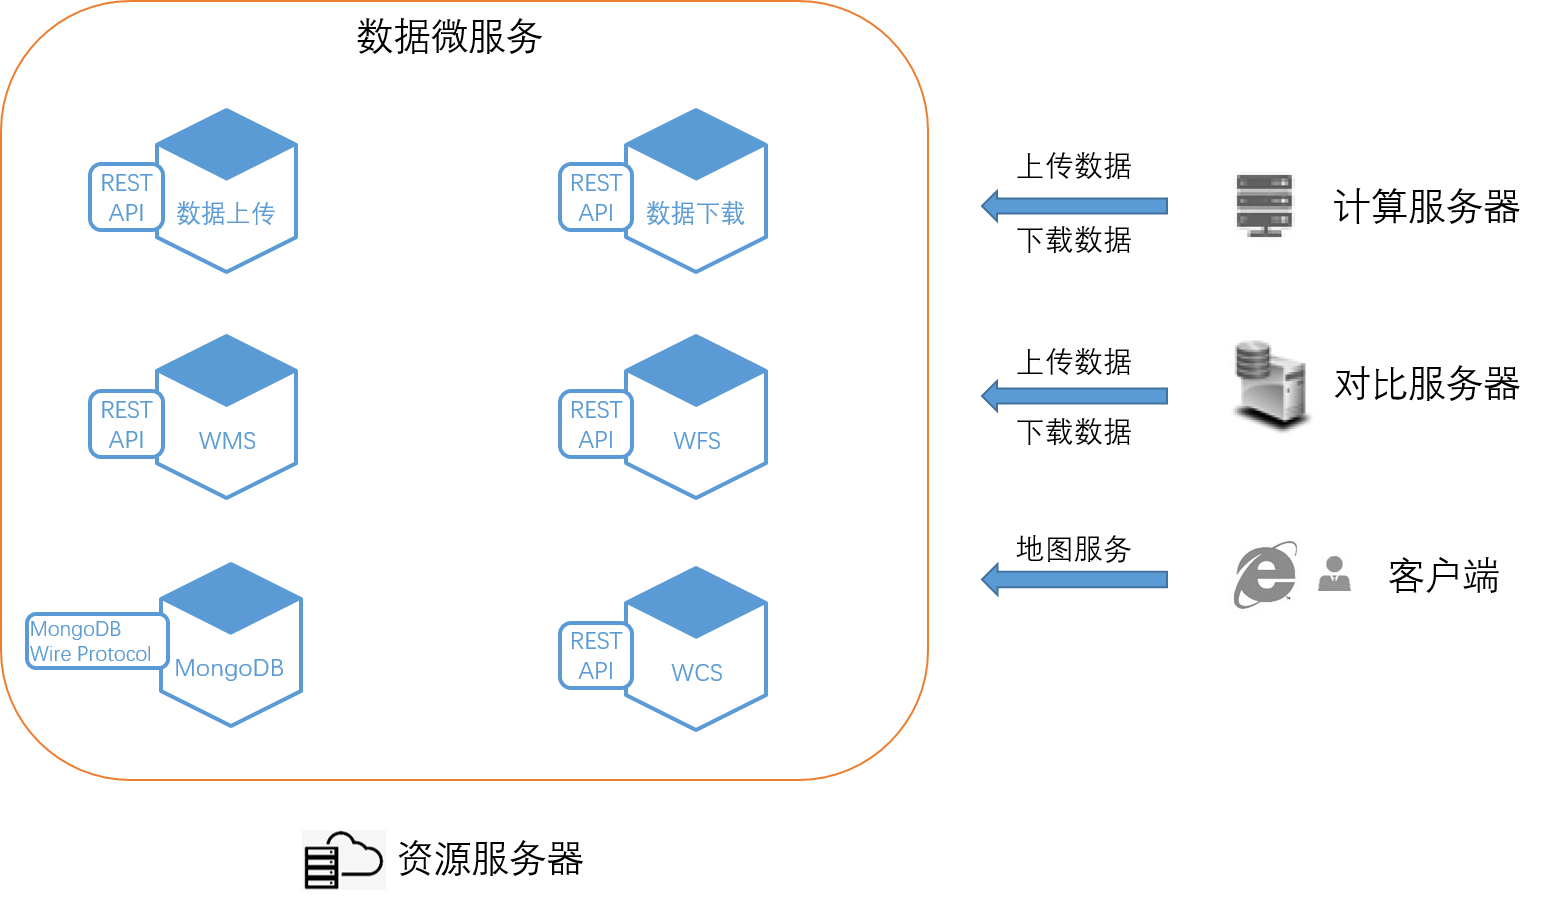
\includegraphics[width=1\textwidth]{resource-server-microservice}
%     \caption{数据管理容器微服务}
%     \label{fig:resource-server-microservice}
% \end{figure}

\subsubsection{模型计算容器}
\begin{figure}[!htbp]
    \centering
    \subcaptionbox{模型微服务的发布和调用}{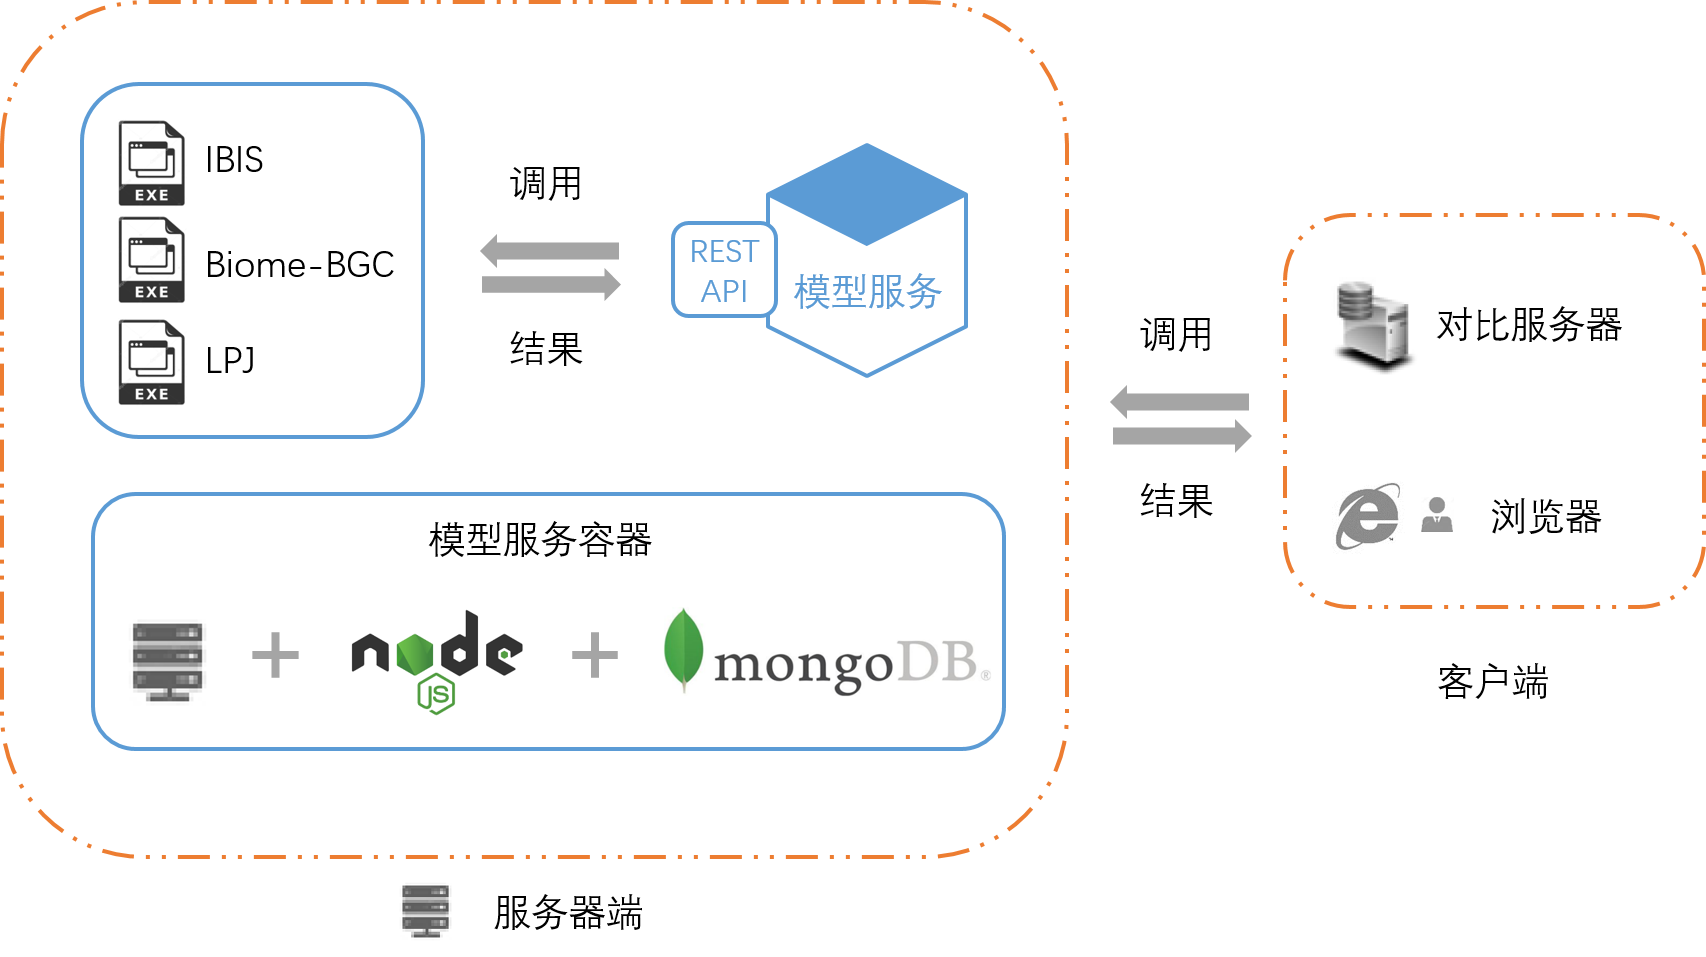
\includegraphics[width=0.65\textwidth]{ms-server-microservice-a}}
    \hfill
    \subcaptionbox{模型微服务多节点分布}{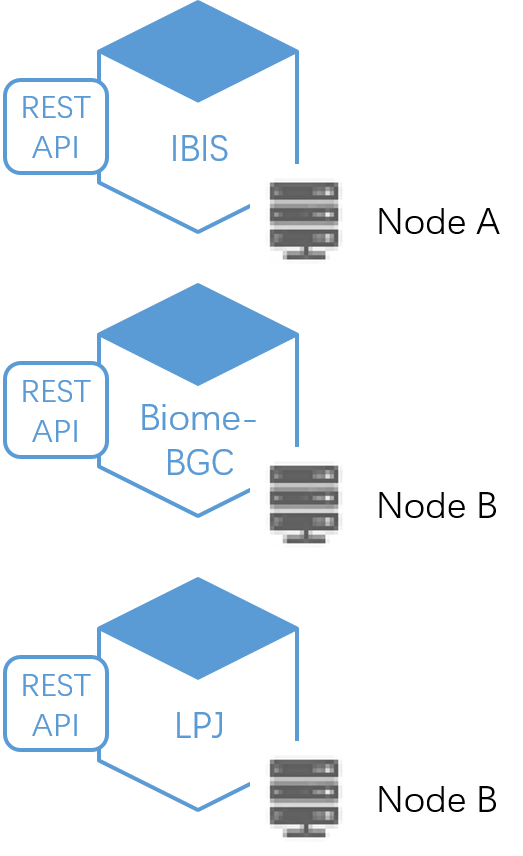
\includegraphics[width=0.25\textwidth]{ms-server-microservice-multi-nodes}}
    \caption{模型计算容器微服务}
    \label{fig:ms-server-microservice}
\end{figure}

模型计算容器的主要功能是模型服务的发布、注册、管理和调用,如图~\ref{fig:ms-server-microservice}所示,模型计算容器由Node.js和MongoDB开发。Node.js对外暴露模型调用的接口,当客户端经过HTTP协议发送调用请求时,在模型计算容器内部调用模型应用程序。当模型运行结束后,模型计算容器获取子程序的句柄,将运行结果的状态保存到MongoDB中。模型微服务与数据微服务有一些不同之处:每个独立的模型服务可以根据软硬件需求存放在不同的服务器上,即模型微服务有多计算节点的特性。因此,模型微服务发布后,还需要将服务注册到模型服务资源库中,从而能够被服务消费者发现服务。

\subsubsection{模型对比容器}
对比服务容器的主要功能是将对比任务中包含的计算任务分发给模型计算容器,并把模型计算出来的结果文件和对比参考数据进行对比。他是模型微服务和数据微服务的消费者、对比微服务的生产者。如图~\ref{fig:compare-server-microservice}所示,模型对比的开展主要包括以下几步:

\begin{enumerate}[(1)]
\item 用户在浏览器客户端通过HTTP协议发送对比任务的调用请求;
\item Node.js的路由器收到请求后,将对比任务中包含的计算任务拆分出来,并通过调用模型计算容器上的模型微服务启动计算任务,并不断轮询监控模型的运行进度;
\item 当监测到所有模型都运行成功后,从数据管理容器上获取模型运行结果和对比参考数据,然后调用本地的对比方法脚本程序,这些脚本可由JavaScript、Python或Matlab等编写而成;
\item 最后将对比脚本的结果文件保存到数据库中,并返回给客户端。
\end{enumerate}

另外他作为门户网站的后台服务器,还负责浏览器前台的一系列操作,如资源汇总与展示、对比流程的创建、对比结果的展示等。

\begin{figure}[!htbp]
    \centering
    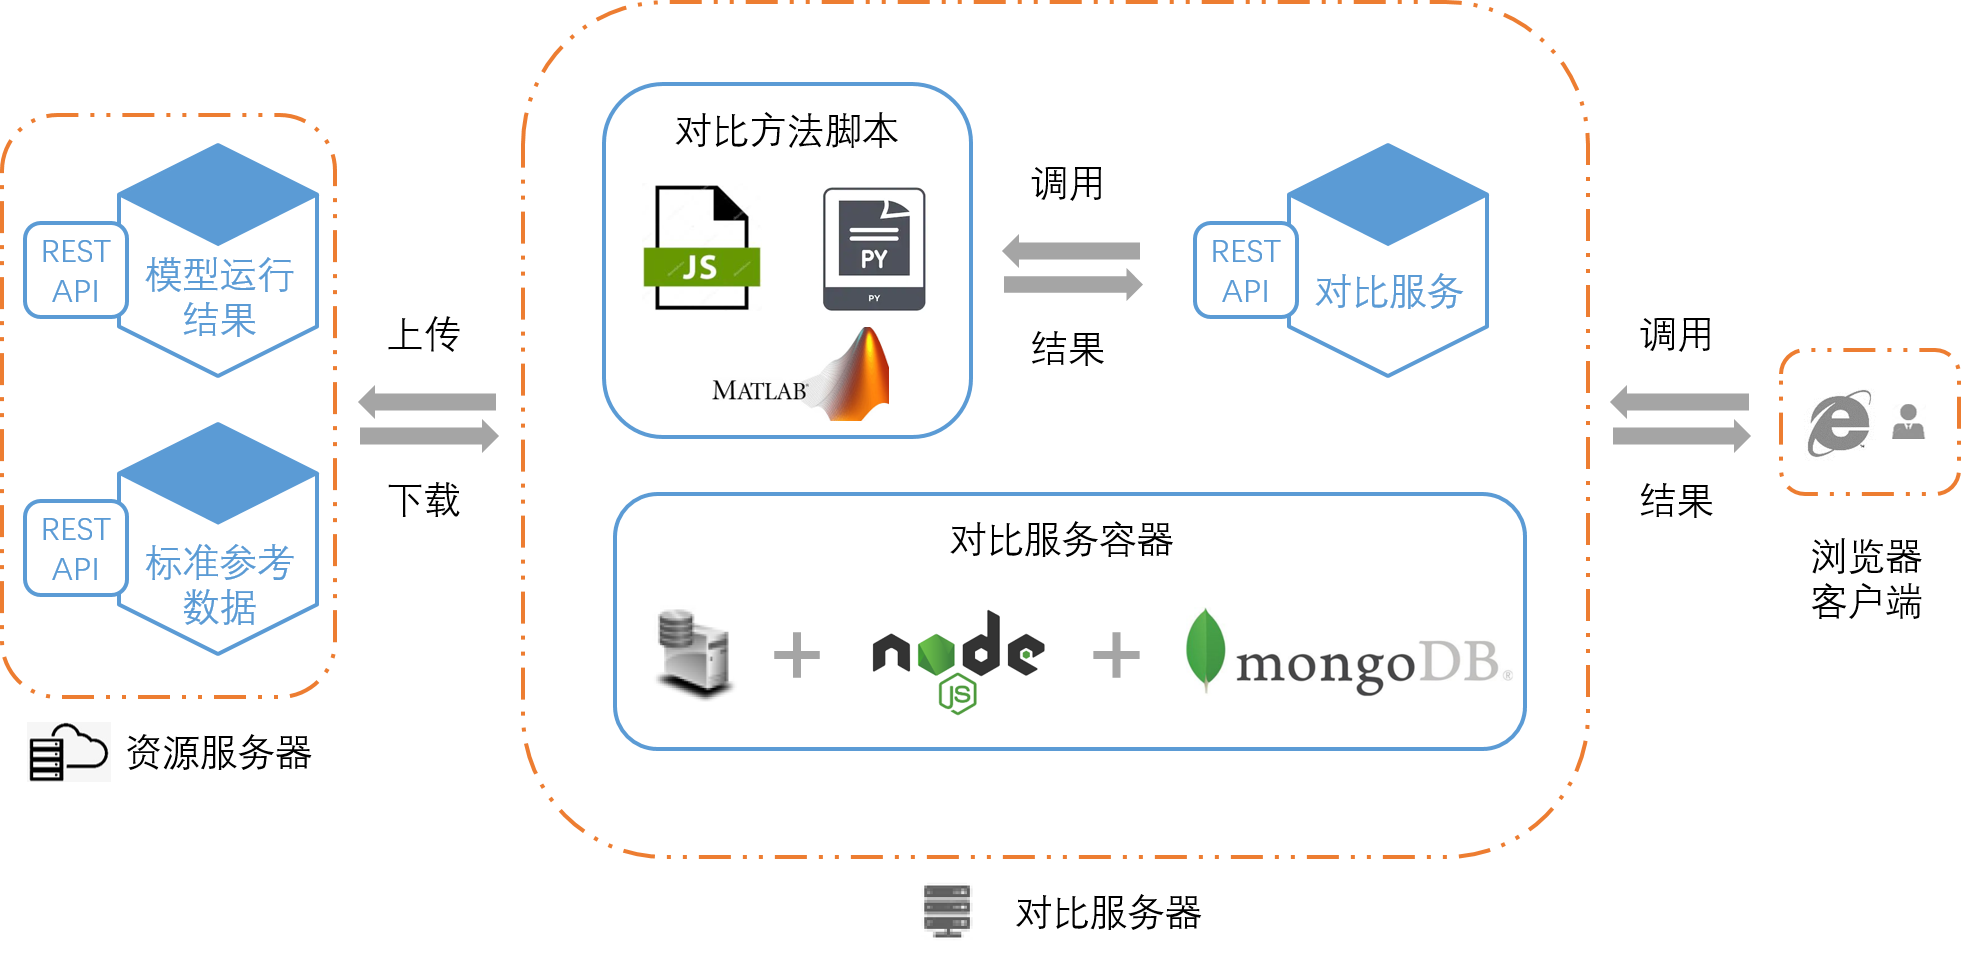
\includegraphics[width=1\textwidth]{compare-server-microservice}
    \caption{对比服务器微服务}
    \label{fig:compare-server-microservice}
\end{figure}

\section{对比科学工作流引擎}
\subsection{对比流程分析和归纳}
图~\ref{fig:workflow-example}展示了传统方法在本地进行对比时的流程,整个流程可以概括为“模型计算——数据重构——结果对比”三步。模型计算过程中对比参与者同时输入数据启动运行;数据重构过程将运算结果转换为标准化数据;结果对比过程使用脚本分析。当加入新的对比参与者时整个对比流程也不会发生变化。

\begin{figure}[!htbp]
    \centering
    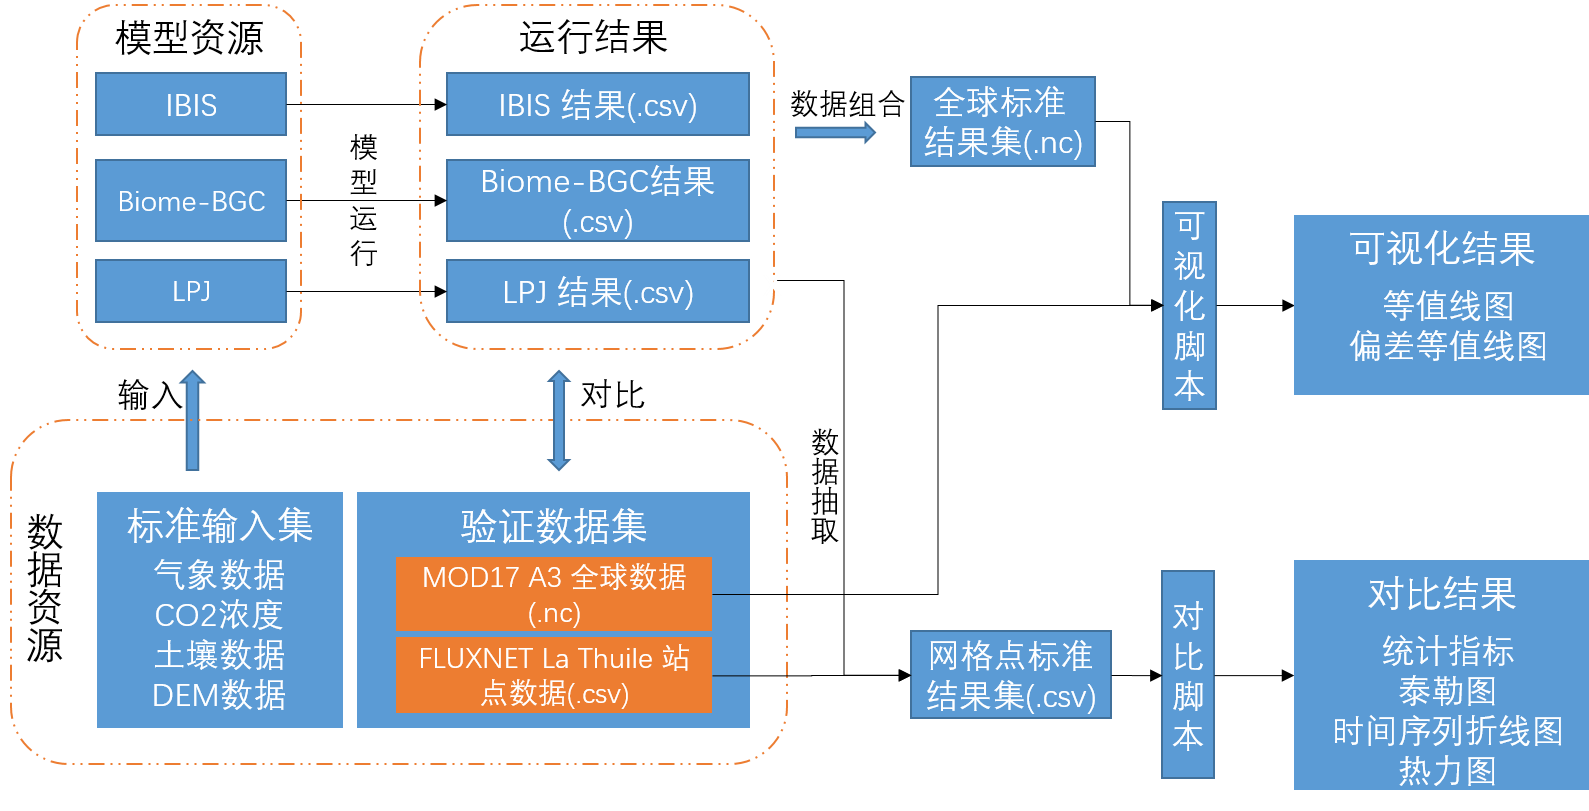
\includegraphics[width=1\textwidth]{workflow-example}
    \caption{以IBIS、Biome-BGC、LPJ三个模型为例的对比流程}
    \label{fig:workflow-example}
\end{figure}

\subsection{对比自动化执行引擎}
%  流程创建:是对工作流过程的抽象表示,定义工作流执行时使用的资源,其依赖关系着重表达了各任务之间从数据生产者到数据消费者的流程,这些资源是指可执行网络服务、数据,对应对比方案
%  通过流程映射形成可执行的工作流实例,对应对比任务
% 工作流定义:工作流语言通常用XML这种形式化描述语言,表达组成流程的任务和任务之间的依赖关系,SWF没有标准语言,流程定义只能由各自的流程引擎解析执行
% 工作流执行:运行时建立网络资源之间的交互关系,将抽象工作流转换成可执行的工作流,建立任务和所需可用资源的映射关系
% 工作流活动之间的依赖主要表达了多个任务之间的逻辑结构和执行方式,包括顺序、并行、循环、条件
在微服务架构下,面临着服务集成的问题,科学工作流是服务集成的一个解决方案。 % 具体化,数据传输的流程
工作流管理联盟(Workflow Management Coalition,WfMC)将工作流定义为一类能够完全或者部分自动执行的经营过程,根据一系列过程规则,文档、信息、或任务能够在不同的执行者之间传递、执行。科学工作流是工作流的一种,它主要面向科学实验过程,以数据驱动,用来描述和控制科学实验和过程的执行~\cite{ludascher2006scientific}~\cite{Zhao2009Special}。

科学工作流的生命周期可归纳为一下三点:
\begin{enumerate}[(1)]
    \item \textbf{流程创建:}定义工作流执行时所参与的活动,以及数据在活动之间的流向关系,在本文中活动是指各种模型服务、数据重构服务和对比服务。定义出的工作流表达了数据从生产者到消费者之间的流向关系,但还不包括数据实体;
    \item \textbf{流程映射:}绑定活动所需要的数据实体,从而将工作流映射为可执行的工作流实例;
    \item \textbf{流程执行:}解析工作流中活动的依赖关系,并在网络环境下进行运算。
\end{enumerate}

在本文的对比流程中,工作流模式固定,如图~\ref{fig:workflow},都是分“模型计算——数据重构——模型对比”三步,所以不再通过图形化界面创建工作流,只需要通过选择对比参与者和对比方法就能够重现出这三部流程,所以本文的工作流通过对比方案表达,流程创建对应对比方案的创建,流程映射对应对比任务的创建,流程执行对应对比任务的执行。

% 每一步都是在网络环境下,有频繁的数据传输交互

\begin{figure}[!htbp]
    \centering
    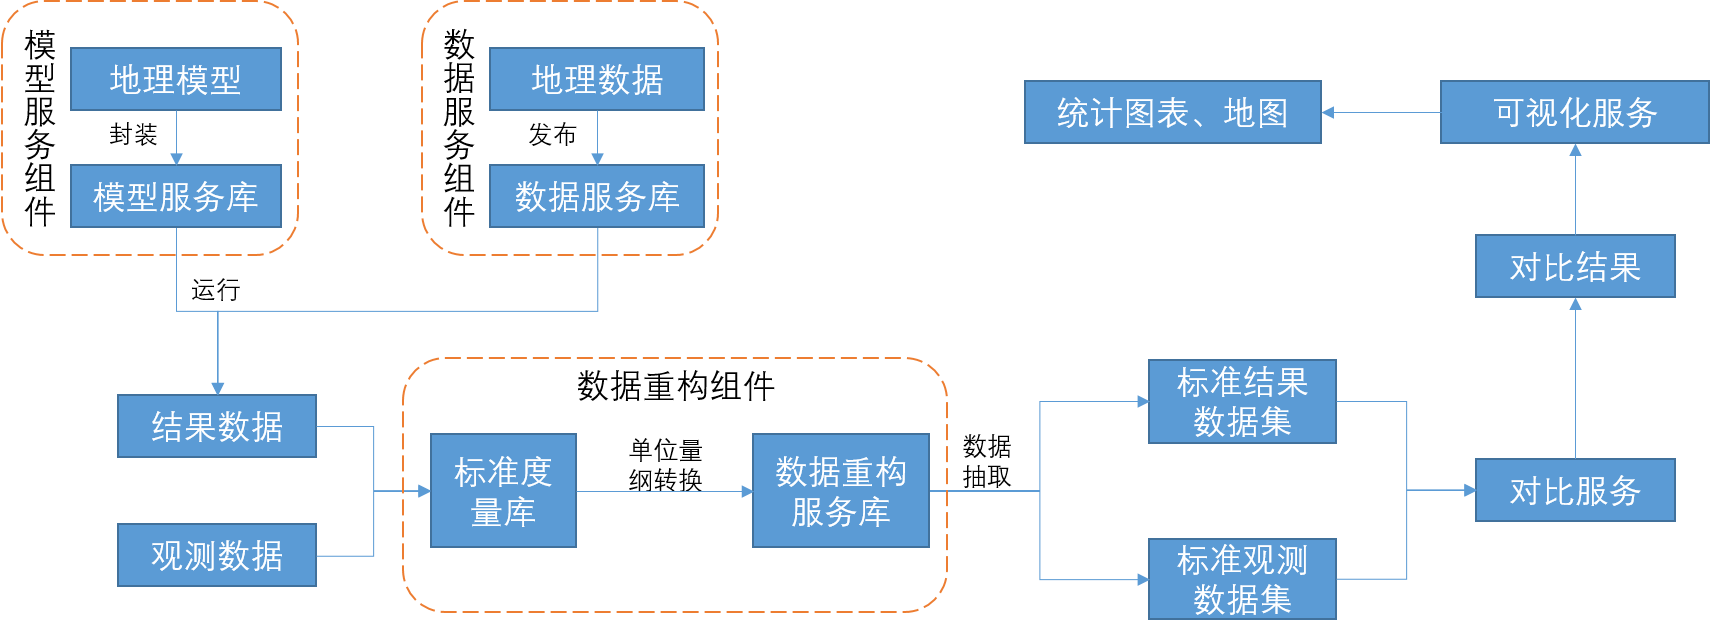
\includegraphics[width=.5\textwidth]{workflow}
    \caption{开放式对比科学工作流流程图}
    \label{fig:workflow}
\end{figure}

\section{本章小结}
开放式对比系统的构建有两个关键问题:一是如何设计一个开放式的对比框架,二是这些对比资源如何接入框架。对于问题一,本章从对比业务、资源组件、网络架构和执行引擎四个角度进行了详细论述,设计的系统框架具有以下特点的:

\begin{enumerate}[(a)]
    \item 模型计算和对比可共享与重用;
    \item 模型计算和对比过程公开化;
    \item 模型和数据资源可扩展性地动态接入;
    \item 大规模计算场景下稳定可用;
    \item 以自动化实现其易用性。
\end{enumerate} 

对于问题二将在下一章详细论述。